\documentclass{acm_proc_article-sp}
\usepackage{float}
\begin{document}

\title{Essence of Context-Oriented Programming}

\author{
\alignauthor
Ivo Willemsen\\
       \affaddr{Open Universiteit}\\
       \affaddr{Maastricht, The Netherlands}\\
       \email{ivo.willemsen@outlook.com}
}

\maketitle
\begin{abstract}
The last decade, use cases have emerged that emphasise the need to cater for different behaviour depending on situation and context changes. Examples are: Pervasive systems \cite{pervasivecomputing} and highly personalised business applications. Conventional programming languages offer constructs to implement context-dependent behavior, like  conditional branches using if/switch statements, but they often result in cluttered code and uses of those 
constructs seriously damage the modularity of the applications. In the early 2000s, a new programming paradigm emerged, called Context-Oriented Programming which targeted to mitigate the aforementioned problems by incorporating context as as part of the programming language, like variables, classes, and functions constitute the constructs 
of many contemporary languages.

This paper presents an introduction to Context-Oriented Programming, focussing on what Context-Oriented Programming is and explaining the \textit{raison d'etre} of its usage. As additonal reading, examples of Context-Oriented Programming languages are given and some other aspects of these languages are elaborated on.  
\end{abstract}

\keywords{Context-Oriented Programming, context-aware systems, behavioural variations} 

\section{Introduction} \label{introduction}
Many applications present behaviour that is determined by the context in which it is being used. Examples of different contexts are: Battery level, GPS location, available connectivity protocols (Wifi/3G/4G), speed of the network, user's preferences, etcetera.

For example, battery level of a tablet or a smartphone on which an application (Operating System in this case) runs is a context, which probably impacts many behavioural aspects of that applications. It will not only have affect on the brightness of the screen, but it might also influence the way the Operating System prioritises running threads, and perhaps result in the preventive hibernation of the system.

In order to include context-dependent behaviour in applications using most modern programming languages, one option available is to use the Strategy Design Pattern \cite{strategypattern} to abstract the context-dependent behaviour into separate classes and decide at runtime-level which context-dependent behaviour (strategy) to use. Even worse would be the usage of conditional statements to find out the context in which a certain program is running, and as a result, not adhering to one of the concepts of Object-Oriented Programming: To avoid conditonal statements to determine polymorphic behaviour. Both options are suboptimal as they result in cluttered code which is difficult to reuse and to understand and makes maintenance of the code a very cumbersome activity.

So, behavioural variation is not implemented by a sole object, rather it is spread over a group of cooperating objects. It is called a crosscutting concern \cite{kiczalesetallaop} and this is a functionality that is dispersed over several cooperating objects. Plain old Object-Oriented Programming languages don't have constructs that allow for modularization and composition of crosscutting concerns, they lack first-class constructs. A first-class construct \cite{Keays:2003:CP:940923.940926} is a construct which is an element of a language, like a class or a method in Java. The lack of first-class constructs in regular Object-Oriented Programming languages to support the development of context-aware applications, leaves the developer of those applications with the need to implement necessary \textit{boiler-plate code}. What is needed, is a type of language that incorporates those constructs; which allow a developer to focus more on the implementation of business use-cases and less on inventing the wheel of "context determination, modularlisation and activation" over and over again. 

Chapter \ref{motivation} will elaborate more on the motivation of the need for a new programming paradigm. Chapter \ref{context} will zoom into the concept of "Context" and dependencies between different contexts. 

\section{Context}\label{context}
Context can be defined as any information that can be used to characterise the situation of an entity. An entity is a person, place or object that is considered relevant to the interaction between a user and an application, including the user and the application themselves \cite{Abowd:1999:TBU:647985.743843}. Context is derived from three sources: Environment, system and the actors. Contextual information that originates from actors and the environment is information that reaches the system from outside, but the system itself can also generate context. 

A \textit{system} is a set of computational objects, methods, functions that responds with pre-defined behaviour on per-request basis. An \textit{actor} is a person or another system that is directly involved with the system: It determines the order in which use cases are executed by communicating direclty with the system, by clicking on buttons, sending messages, receiving feedback, etcetera. An example of context generated by an actor is the differences in behaviour that originate from the choices made by a user when accessing certain functionalities. Another example is the support of multiple devices (like an smartphone or a desktop computer) that add to the context-dependent behaviour of the system. The \textit{environment} encompasses everthing that lies outside the boundaries of the system, and which is not directly involved in the relationship between the system and the actors.

behaviour variations, changes in response, depend on context or a combination of contexts that is generated by these three sources. as a result, context-dependent behaviour variations can be divided into actor-dependent, environmentent-dependent and system-dependent variations.

\section{Context-Oriented Programming}\label{cop}
In the early 2000s, a new programming paradigm appeared which is called COP (Context-Oriented Programming). This development was triggered by the appearance of a wide range of scenarios where applications had to react differently according to the active context. Conventional Object-Oriented Programming languages did not exhibit language structures that enabled developers to code behavioural variations to changes in contexts in a moduluar way. 

Context-Oriented Programming promotes the modularisation of context-dependent behavioural variations. It offers exclusive abstractions and mechanisms in the form of first-class constructs which enables developers to effectively define entities that need to change behaviour depending on their context. It allows applications to be partitioned into behavioural variations that can be activated at runtime level with pre-defined scopes. These behavioural variations are composed of of \textit{partial definitions} for entities, like classes, functions, methods, procedures, etcetera. Context-oriented Programming offer the following functionalities whose mechanisms are implemented as part of the language \cite{Costanza:2008:CPC:1529966.1529970}:

\begin{itemize}
\item {Context}
\item Behavioral variations
\item Layers
\item Layer activation
\item Scoping
\end{itemize}

\textit{Context} is information that can be computationally accessed in a software system. This information is part of the context on which behavioural variations depend. This definition is kind of vague, as it leaves room for a variety of interpretations: 
\begin{itemize}
\item The definition does not specify whether the information should originate from outside of the system, the environment, but is also comes from other sources like the actors and the system itself.
\item The granularity of abstraction is not enforced by the definition. Context can exist in the system, or can come to the system as fine-grained pieces of information, like indiscrete numerical temperature indications and can subsequently be transformed to more course-grained information classes like "low", "medium", "high". 
\item The uniqueness of the context is not imposed. There exist implementations of Context-Oriented Programming languages that enable applications to share only a common context. Other implementations don't follow this model and allow several contexts to exist, which are used in different parts of the application \cite{Appeltauer:2009:CCP:1562112.1562118}
\end{itemize}

Context-Oriented Programming languages have first-class constructs that support \textit{behavioural variations} by means of partial definition of modules. Behavioural variations can be expressed in terms of new behaviour, modified behaviour or behaviour that has been removed. The first-class constructs that are involved in these concepts are plain Object-oriented Programming constructs like classes and methods. Behavioural variations can be \textit{activated}, partly changing the behaviour of the application. So, the function of behaviour variations is to allow \textit{runtime activation} of a change in behaviour, and it also allows for the \textit{modularisation} of behaviour by exploiting the available constructs in the Context-Oriented Programming language.    

\textit{Layers} group contextual-dependent behavioral variations as first-class entities that can be explicitly referred to in a program at runtime. Layers are first-class entities in most Context-Oriented Programming languages, which groups partial definitions and can be stored in variables and passed to methods. Several part of the application can have access to the same layers and determine the exact changes in behaviour that have to be done. In case of layers, the first-class entity that implements this functionality is a layered method. This method consists of a base, principle method definition, extended with at least one extra partial definition.

\textit{Layer activation} is achieved by language constructs that
ensure that such layers are added at runtime, such that
the respective partial program definitions have an in-
fluence on the actual behavior of a program.

\textit{Scoping} of layer activation and deactivation ensures that
the behavioral variations are only effective for welldefined
parts of a program, and for well-defined durations.

fdsfdsfd
 
\begin{figure}[H]
\centering
\fbox{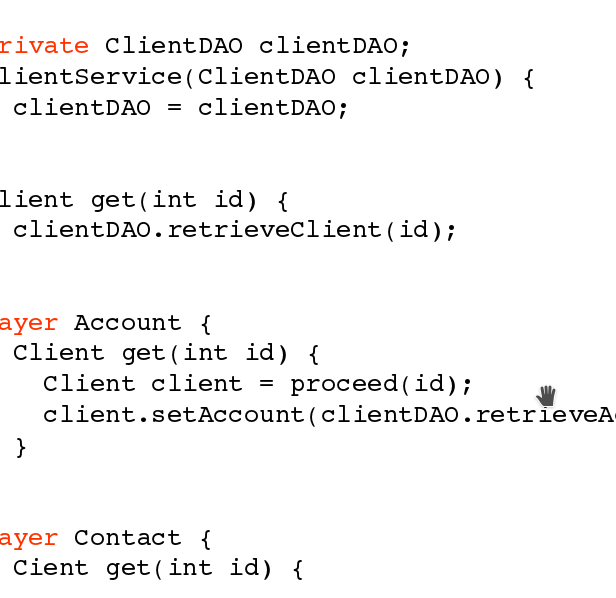
\includegraphics[width=40mm]{pic.png}}
\caption{Definition of layers}
\end{figure}

ref no 6.!!!1 relationship between activation and beh var.


\bibliographystyle{abbrv}
\bibliography{sigproc}
\end{document}
